% ============================================================
\chapter{本プロジェクトの LLM のビューで確かめる}\label{ch:project}

この章では、ここまでのコツを本プロジェクトのデータに当てはめる。LLM の予想の当たり具合を測り、回答のばらつきと実際の外れを比べ、$\Omega$ の決め方を 7 通りに変えて 30 か月の比率を計算し直す。

\section{データと設定}

\begin{itemize}
\item \textbf{LLM の回答}：実行番号 1（gpt-4o-mini、温度 1.0、1 銘柄あたり 30 回）。判断日は 2024 年 3 月 28 日〜2026 年 8 月 31 日の各月末の \V{llm.months} 回。各判断日の \SP{} の構成銘柄について、その月の日次リターンを渡し、翌月の日次の平均リターンを答えさせた。
\item \textbf{実際の結果}：判断日の翌月の日次リターンの平均（15 日以上のデータがある銘柄）。銘柄と月の組は \V{llm.rows} 個。
\item \textbf{BL}：本プロジェクトのコード（\code{blm/}）をそのまま使う。共分散は過去 252 取引日の縮小推定、$\delta=\V{blm.delta}$、$\tau=\V{blm.tau}$、$P=I$、最適化は空売りなし・全額投資。
\end{itemize}

\section{当たり具合}

\begin{table}[htbp]
\centering
\caption{判断日ごとの当たり具合。順位相関と相関は予想と翌月の実際の相関、傾き $b$ は実際を予想に回帰した傾き、入力との相関は予想と渡した月の平均リターンの相関、右端は回答の分散 ÷ 誤差の 2 乗の中央値。}
\label{tab:llm-monthly}
\small
\tabin{llm_monthly}
\end{table}

\begin{figure}[htbp]
\centering
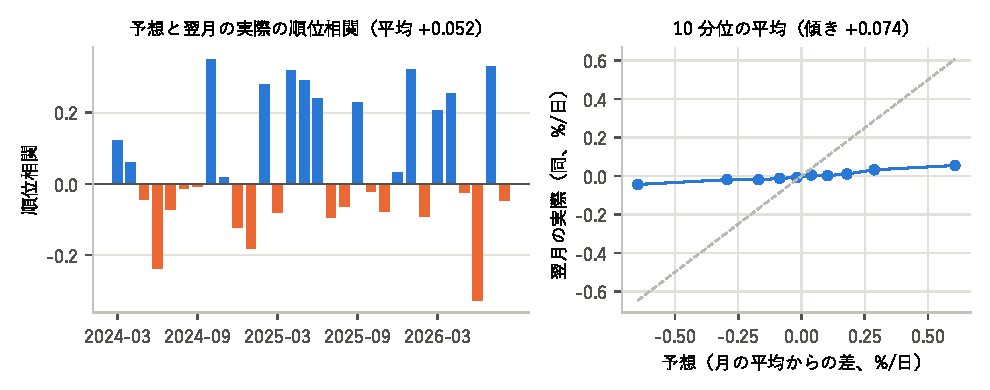
\includegraphics[width=0.95\linewidth]{fig_llm_ic.pdf}
\caption{左：判断日ごとの、予想と翌月の実際の順位相関。右：判断日ごとに平均を引いた予想の 10 分位ごとの、翌月の実際（同じく平均を引いたもの）。破線は 45 度の線。}
\label{fig:llm-ic}
\end{figure}

\tabref{tab:llm-monthly} と\figref{fig:llm-ic} から分かることを挙げる。

\begin{itemize}
\item 順位相関の平均は \V{llm.ic.mean}（$t$ 値 \V{llm.ic.t}、30 か月のうちプラスは \V{llm.ic.pos} か月）。相関（Pearson）の平均は \V{llm.icp.mean}。値としては、優れた運用者の目安（0.05 前後）と同じくらいだが、偶然と区別できるほどではない。
\item 傾き $b$ の平均は \V{llm.slope.mean}（$t$ 値 \V{llm.slope.t}）、30 か月をまとめると \V{llm.slope.pooled}。予想の散らばりのうち、翌月の差につながっているのは 7\% 程度である。\figref{fig:llm-ic} の右の 10 分位の点は、45 度の線よりずっと寝ている。
\item 予想と渡した月の平均リターンの相関は \V{llm.cin.mean}。予想は、ほぼ先月の値動きの写しである（『総合報告書』問題 2）。
\end{itemize}

予想の散らばり（判断日ごとの標準偏差の平均）は日次 \V{llm.sdQ}\%、実際の翌月の平均リターンの散らばりは \V{llm.sdr}\% で、大きさは近い。しかし、相関が 0.05 程度なので、予想を期待リターンとしてそのまま使うと、十数倍の自信過剰になる（傾き 0.07 の逆数は約 14）。

\section{回答のばらつきと、実際の外れ}

\begin{figure}[htbp]
\centering
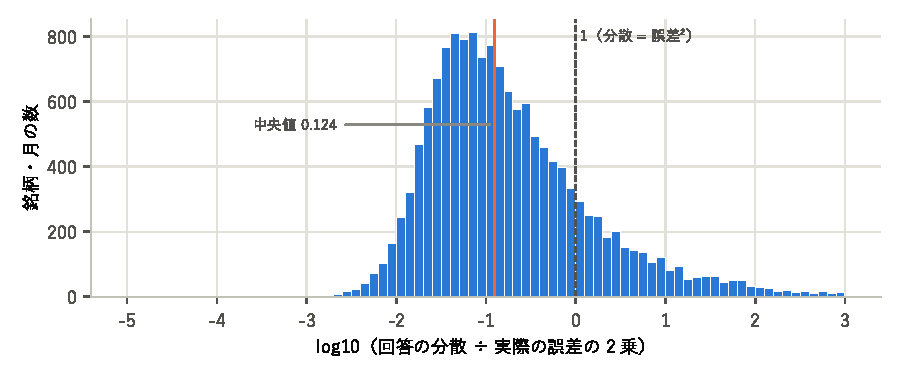
\includegraphics[width=0.92\linewidth]{fig_llm_ratio.pdf}
\caption{回答の分散 ÷ 実際の誤差の 2 乗（銘柄・月ごと、対数）。1（破線）なら、ばらつきが外れの大きさと合っている。}
\label{fig:llm-ratio}
\end{figure}

回答の分散と、実際の予想の外れ（予想 $-$ 翌月の実際）の 2 乗の比は、中央値で \V{llm.ratio.med}、四分位で \V{llm.ratio.q25}〜\V{llm.ratio.q75} だった（\figref{fig:llm-ratio}）。回答の標準偏差の中央値は日次 \V{llm.omsd}\% で、実際の外れ（誤差の 2 乗の平均の平方根で日次 0.6\% 前後）よりずっと小さい。

\chapref{ch:accuracy} の式~\eqref{eq:omega-err} で、避けられない外れ（翌月の日次リターンの平均そのものの散らばり）を差し引いても、外れの分散は回答の分散の平均の 5 倍以上だった。回答のばらつきを $\Omega$ にすると、外れを 5〜8 分の 1 に見積もることになる。

\section{1 銘柄で見た採用率}

回答の分散を、$\tau\Sigma$ の対角（$\tau=0.025$、過去 1 年の日次の分散）と比べると、比の中央値は \V{llm.omtau.med} で、1 銘柄だけで見た採用率は \V{llm.adopt.med}\% になる（\chapref{ch:overview} の\figref{fig:adoption}）。当たり具合から見た妥当な採用率（傾き 0.07 程度）の 10 倍以上である。

\section{$\Omega$ の決め方を変えて計算し直す}

$\Omega$ の決め方を次の 7 通りにして、30 か月の比率を計算し直した。

\begin{enumerate}
\item \textbf{回答の分散（元の方法）}：$\Omega=\diag(\text{回答の分散})$。本プロジェクトの「直した計算」と同じ。
\item \textbf{He--Litterman}：$\Omega=\tau\diag(\Sigma)$。1 銘柄なら採用率 50\%。
\item \textbf{傾きで較正（対角）}：$\Omega=\tau\diag(\Sigma)(1/b_t-1)$。1 銘柄なら採用率 $b_t$。
\item \textbf{傾きで較正（$\Sigma$ に比例）}：$\Omega=\tau\Sigma(1/b_t-1)$。どの銘柄も採用率 $b_t$ で、$\muBL=\Pi+b_t(Q-\Pi)$。
\item \textbf{同上 ＋ TE \V{bt.te.target}\% 以内}：4 と同じ期待リターンで、事前の TE を年率 \V{bt.te.target}\% 以内に制限する。
\item \textbf{相対ビュー ＋ TE \V{bt.te.target}\% 以内}：予想と均衡から、それぞれの時価総額加重の平均を引いた差だけを使い（$\muBL=\Pi+b_t[(Q-\wmkt\T Q)-(\Pi-\wmkt\T\Pi)]$）、5 と同じ TE の上限を置く。
\item \textbf{時価総額加重}：ベンチマーク。
\end{enumerate}

$b_t$ は、判断日 $t$ より前に結果が分かっている月だけで計算した傾き（月ごとに平均を引いてまとめる）で、0〜1 に収めた。最初の数か月はデータがなく、$b_t=0$（均衡のまま）である。30 か月のうち \V{bt.b.zero} か月が $b_t=0$ で、最後の判断日の $b_t$ は \V{bt.b.last} だった。

\begin{table}[htbp]
\centering
\caption{$\Omega$ の決め方と、30 か月の比率の性質と成績（年率 \%）。採用率は銘柄ごとの $(\muBL-\Pi)/(Q-\Pi)$ の中央値、実質銘柄数は $1/\sum w^2$ の平均、指数との差は $\frac12\sum|w-\wmkt|$ の平均、TE・IR は時価総額加重に対する実績、回転率は月平均。}
\label{tab:blm-omega}
\tabin{blm_omega}
\end{table}

\begin{figure}[htbp]
\centering
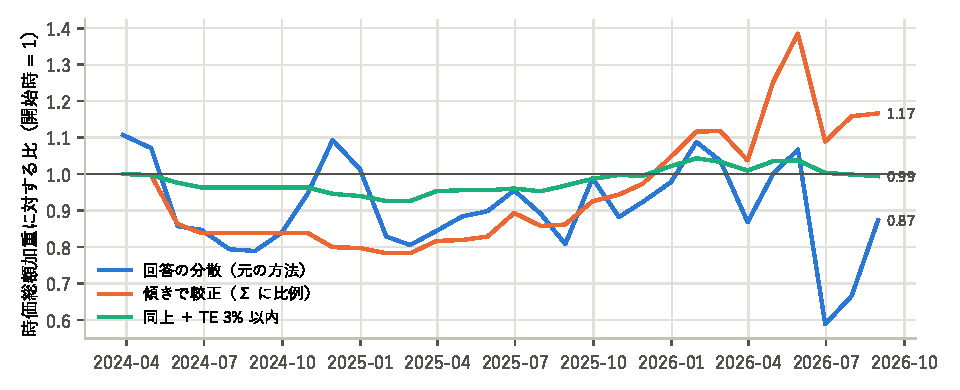
\includegraphics[width=0.95\linewidth]{fig_blm_omega.pdf}
\caption{時価総額加重に対する累積の比（30 か月）。}
\label{fig:blm-omega}
\end{figure}

\begin{figure}[htbp]
\centering
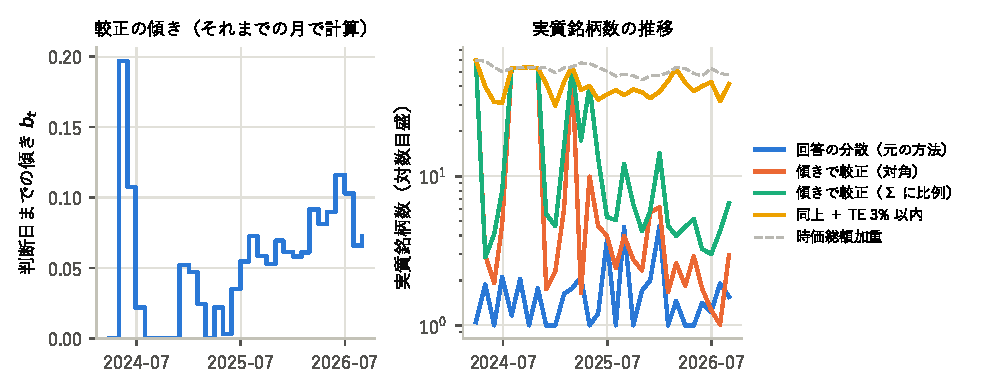
\includegraphics[width=0.98\linewidth]{fig_blm_omega_time.pdf}
\caption{左：判断日までに分かっている月だけで計算した較正の傾き $b_t$。右：比率の実質銘柄数の推移（対数目盛）。}
\label{fig:blm-omega-time}
\end{figure}

\figref{fig:blm-omega-time} の左のとおり、較正の傾き $b_t$ は、最初の 2 か月はデータがないので 0 である。結果が 1〜2 か月分しかない時期には 0.2 まで跳ね、その後しばらくは負の傾きを 0 に切り上げた 0 が続き、2025 年の半ば以降は 0.05〜0.12 の範囲に落ち着いた。少ない月から推定した傾きは大きく揺れるので、データが少ないうちは 0 に寄せて使うほうがよい（\secref{sec:slope}）。

右のとおり、回答の分散を $\Omega$ にした元の方法では、比率は毎月 1〜4 銘柄に集中する。較正した版は、$b_t=0$ の月には均衡のままなので時価総額加重と同じ比率（約 50 銘柄）になり、$b_t$ が正の月には、対角の $\Omega$ では数銘柄、$\Sigma$ に比例させても数銘柄〜十数銘柄に集中する。TE の上限を付けると、どの月も 30〜50 銘柄に収まる。採用率を正しく縮めても、TE の上限がなければ比率は集中する、ということが月ごとにも確かめられる。

\section{結果の読み方}

\tabref{tab:blm-omega} と\figref{fig:blm-omega} の読み方を、$\Omega$ の決め方ごとに述べる。

\begin{description}[leftmargin=2em,style=nextline]
\item[回答の分散・He--Litterman] 採用率は中央値で \V{bt.sample.adopt}\%、\V{bt.hl.adopt}\%。比率は実質 \V{bt.sample.effn}〜\V{bt.hl.effn} 銘柄に集中し、TE は年率 50\% 前後になった。BL というより、LLM の予想をそのまま期待リターンにした平均分散最適化で、成績は集中の結果である。He--Litterman の「ビューと均衡を半々」でも、約 490 銘柄を対角の $\Omega$ で入れると、採用率は 50\% を大きく超える。
\item[傾きで較正（対角）] 1 銘柄なら採用率 5〜7\% のはずが、中央値は \V{bt.calib.adopt}\% になった。約 490 個のビューの外れを独立と扱ったため、全体の水準（その月の予想の平均）への確信が積み上がった（\secref{sec:diag-trap}）。比率は実質 \V{bt.calib.effn} 銘柄、TE は \V{bt.calib.te}\% で、まだ大きい。
\item[傾きで較正（$\Sigma$ に比例）] 採用率は設定どおり \V{bt.full.adopt}\% になった。比率は実質 \V{bt.full.effn} 銘柄まで分散したが、TE は \V{bt.full.te}\% と、まだ大きい。期待リターンのずれが正しく縮められても、$\delta=2.5$ の平均分散最適化は、個別の銘柄に大きく賭ける。
\item[TE \V{bt.te.target}\% 以内] 比率は実質 \V{bt.fullte.effn} 銘柄で、時価総額加重（51.5 銘柄）に近づいた。年率リターンは \V{bt.fullte.ann}\%（時価総額加重は \V{bt.mkt.ann}\%）、リスクとシャープレシオも時価総額加重とほぼ同じになった。実績の TE は \V{bt.fullte.te}\% で、事前の目標を上回った（\secref{sec:te-project}）。
\item[相対ビュー ＋ TE] 結果は、5 の版とすべての指標で同じになった。$\Omega\propto\Sigma$ のもとでは、相対ビューとの違いは全銘柄の期待リターンへの一律の上乗せだけで、全額投資の制約があれば比率は変わらないからである（\chapref{ch:shape}）。採用率の列が \V{bt.relte.adopt}\% と小さく見えるのは、全体の水準の分を除いた差で測っているためである。全体の水準の癖が比率に効くのは、$\Omega$ が対角の場合（上の 1〜3）で、そこでは楽観・悲観が高ベータ・低ベータの銘柄への傾きとして現れる仕組みになっている。
\end{description}

\begin{notebox}[成績の差は偶然と区別できない]
30 か月の超過リターンの $t$ 値は、どの方法でも絶対値で 0.6 未満だった（較正・$\Sigma$ 比例で \V{bt.full.tstat}、TE 制約つきで \V{bt.fullte.tstat}）。この表から「どの方法が勝つか」は言えない。言えるのは、$\Omega$ の決め方で、採用率、集中、TE という比率の性質が大きく変わる、ということである。
\end{notebox}

\section{なぜ較正しても TE が大きいのか}

較正した採用率 5.6\% で、期待リターンのずれはどれくらいになるか。予想のずれ $Q-\Pi$ の散らばりは日次 0.35\% 程度（年率に直すと 80\% を超える）なので、5.6\% を掛けても年率で 5\% 前後のずれが残る。個別の銘柄の年率の特異リスクを 25\% とすると、制約のない最適化の能動的な比率は、1 銘柄あたりおおよそ $\alpha/(\delta\sigma^2)=0.05/(2.5\times0.0625)\approx30\%$ になる。数百の銘柄に、このような大きさの賭けが並べば、空売りなしの制約があっても TE は大きくなる。

つまり、$\delta=2.5$ は「市場全体のリスク」への回避度としては妥当でも、「ベンチマークからのずれ」への回避度としては小さすぎる。能動運用では、ずれへの回避度を別に（ずっと大きく）置くか、TE の上限を置く必要がある（\chapref{ch:te}）。

\section{限界}

\begin{itemize}
\item \textbf{期間が短い}：30 か月では、IC が 0.05 程度の予想の価値は確かめられない（\chapref{ch:accuracy} の推定の誤差）。
\item \textbf{モデルが 1 つ}：gpt-4o-mini だけである。対象論文のように複数のモデルで違う「スタイル」が出るかは、この比較では分からない。
\item \textbf{傾きの推定}：$b_t$ は少ない月から推定しており、最初の数か月は 0 だった。データがたまれば安定するが、それまでは 0 に寄せた値を使うのが安全である。
\item \textbf{取引費用}：この比較には入れていない。回転率は月 60〜100\% と大きく、費用を入れると成績はさらに下がる。
\item \textbf{先読み}：gpt-4o-mini の学習データの締め切り（2023 年 10 月）は、判断日（2024 年 3 月以降）より前である。ただし、構成銘柄の選び方などの先読みは『総合報告書』の議論のとおりで、ここでは扱っていない。
\end{itemize}

\section{本プロジェクトへの提案}

\begin{enumerate}
\item \textbf{較正の仕組みを組み込む}：DB には予想（\code{llm\_views}）と株価がそろっているので、判断日ごとに、それまでの月の傾き $b_t$（と IC）を計算して保存する。$\Omega$ はこの $b_t$ から決める。
\item \textbf{$\Omega$ を $\Sigma$ に比例させる}：$\Omega=\tau\Sigma(1/b_t-1)$ にすれば、事後の期待リターンは $\Pi+b_t(Q-\Pi)$ で、採用率が設定どおりになる。対角の $\Omega$ は使わない。
\item \textbf{相対ビューにする}：予想から判断日ごとの平均を引き、全体の水準の癖（楽観・悲観）を取り除く（\chapref{ch:shape}）。$\Omega\propto\Sigma$ と全額投資の組み合わせなら自動的に打ち消されるが、$\Omega$ を対角にする場合や、制約を変える場合に備えて、ビューの段階で取り除いておくのが安全である。
\item \textbf{TE の上限を置く}：事前の TE の上限を置く。実績が目標を上回るので、事前の目標は控えめにする。
\item \textbf{設定を変えたら較正し直す}：温度、質問、モデルを変えると、予想の散らばりも当たり具合も変わる。
\item \textbf{評価の指標}：成績（リターン）だけでなく、IC、傾き、回答の分散と誤差の比、採用率、実質銘柄数、TE を毎回記録する。
\end{enumerate}

\begin{keybox}[この章のまとめ]
\begin{itemize}
\item LLM の予想の当たり具合は、順位相関 \V{llm.ic.mean}、傾き \V{llm.slope.pooled} で、弱い正だった。
\item 回答の分散は、実際の外れの 2 乗の中央値の \V{llm.ratio.med} 倍で、予想を 8 倍前後信じすぎる設定になる。
\item $\Omega$ を傾きで較正し、$\Sigma$ に比例させると、採用率は設定どおり（\V{bt.full.adopt}\%）になった。対角のままだと \V{bt.calib.adopt}\% に積み上がった。
\item 較正しても、平均分散最適化は大きな TE を取る。TE の上限を置くと、比率は時価総額加重に近づいた。
\item 30 か月では、成績の差は偶然と区別できない。
\end{itemize}
\end{keybox}
